%!TEX root = ../sbc-template.tex

%conceito, inspiração biológica
Redes Neurais Artificiais (RNAs) são um modelo de computação não algorítmica caracterizado por sistemas que, em algum nível, lembram a estrutura do cérebro humano. São sistemas pararelos distribuídos compostos por unidades de processamento simples, os neurônios, que calculam funções matemáticas, normalmente não-lineares. Estes neurônios são dispostos em uma ou mais camadas e interligados por um grande número de conexões normalmente unidirecionais e comumente associadas a pesos que armazenam o conhecimento representado no modelo e ponderam a entrada recebida por cada neurônio da rede. Os principais atrativos das RNAs envolvem a capacidade de capturar tendências a partir de um conjunto de exemplos e dar respostas coerentes para dados não-conhecidos, ou seja, de generalizar a informação aprendida.

A motivação para a criação deste modelo vem do funcionamento do cérebro biológico, que é formado por neurônios interligados que se comunicam entre si de modo contínuo e paralelo através de impulsos nervosos. Esta complexa rede neural biológica é capaz de reconhecer padrões e relacioná-los, produzir emoções, pensamentos, percepcção e cognição, além do . Cada neurônio é composto de um corpo, dendritos e um axônio, como é mostrado na Figura \ref{fig:neuronio_biologico}. Os dendritos são responspaveis pela recepção de impulsos nervosos vindos de outros neurônios; o corpo combina os sinais recebidos pelos dendritos e caso o resultado ultrapasse determinado limiar de excitação do neurônio, são gerados novos impulsos nervosos, que são transmitidos pelo axônio até os dendritos dos neurônios seguintes. Esta conexão unilateral entre neurônios biológicos está expressa na Figura \ref{fig:redeneuralbiologica}.

\begin{figure}[ht]
	\centering
	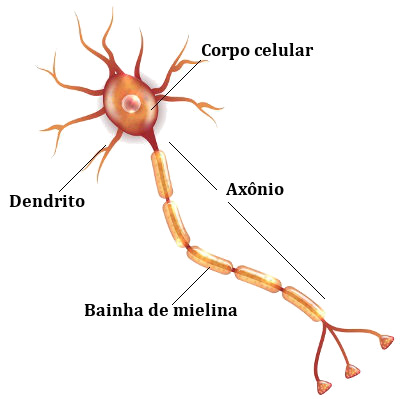
\includegraphics[height=0.3\textheight]{img/neuronio}
	\caption{Neurônio biológico e seus componentes: corpo, axônio e dendritos.}
	\label{fig:neuronio_biologico}
\end{figure}

\begin{figure}[ht]
	\centering
	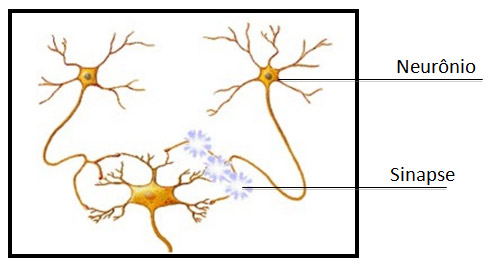
\includegraphics[width=0.6\textwidth]{img/redeneuralbiologica.jpg}
	\caption{Conexão entre neurônios biológicos}
	\label{fig:redeneuralbiologica}
\end{figure}

\begin{figure}[ht]
	\centering
	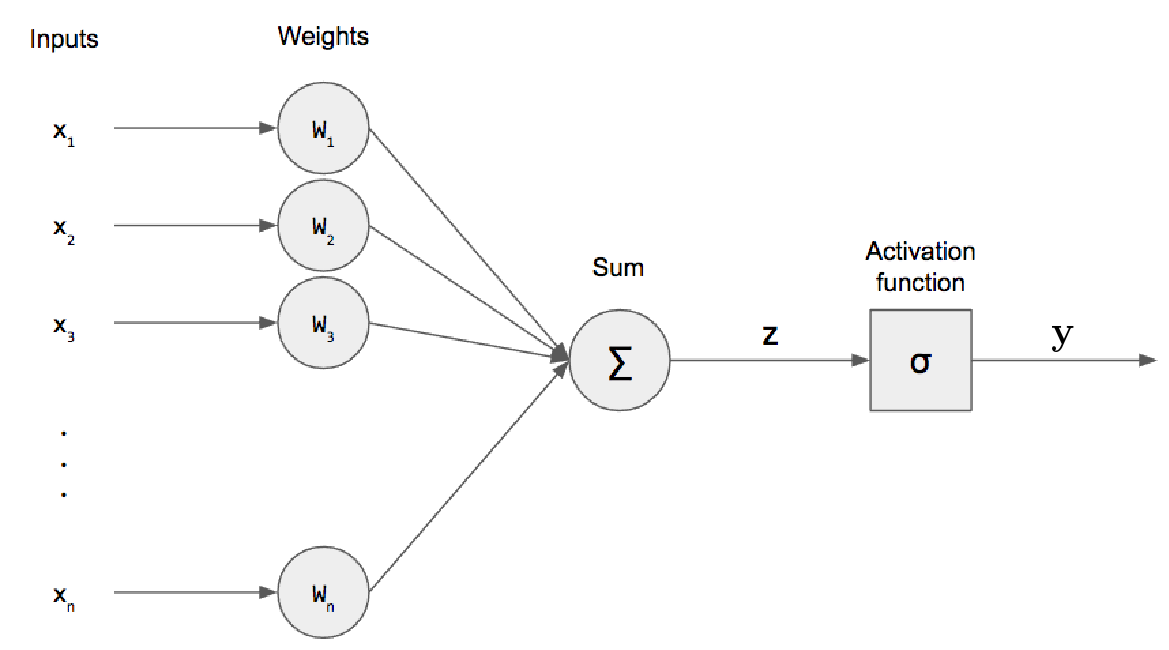
\includegraphics[width=0.7\textwidth]{img/perceptron.png}
	\caption{Representação de um neurônio}
	\label{fig:neuronio}
\end{figure}

Com base neste modelo biológico, McCulloch e Pitts propuseram em \cite{mcculloch1943logical} um neurônio artificial. Explanado na Figura \ref{fig:neuronio}, o modelo de McCulloch e Pitts é formado por somente um neurônio artificial que contém $n$ terminais de entrada dada por $ x = x_1, \ldots, x_n$ e um terminal de saída $y$. Esta organização faz uma alusão aos dendritos, centro e axônio de um neurônio biológico. A saída é mapeada através de uma função de ativação $y = g(z)$ expressa na Equação \ref{eq:funcao_neuronio}, em que a soma ponderada $z$ do vetor de entrada $x$ pelo conjunto de pesos $w = w_1, \ldots, w_n$ deve ser maior ou igual a um limiar de ativação $\theta$.

\begin{gather}\label{eq:funcao_neuronio}
	z = \sum_{i=1}^n x_i w_i\\
	y = g(z) =
		\begin{cases}
			0, & \text{se } z < \theta\\
			1, & \text{se } z \geq \theta
		\end{cases}
\end{gather}

Em 1958, Frank Rosenblatt apresenta o neurônio \emph{Perceptron} \cite{rosenblatt1958perceptron}, que mais tarde seria empregado como a unidade de processamento de uma RNA e de outros modelos de ML como as \emph{support vector machines}. O Perceptron agregou ao neurônio de McCulloch e Pitts conceitos cruciais para a caracterização das RNAs como são conhecidas hoje, como a não obrigatoriedade de igualdade dos pesos e limiares de ativação, a possibilidade de os pesos serem positivos ou negativos, a diversidade de funções de ativação, entre outros. Sua maior contribuição envolve a adição de um algoritmo de aprendizado, que permite a adaptação de seus pesos para que a rede possa se aproximar de uma função que exiba saídas adequadas para determinada tarefa de aprendizado dadas as entradas do conjunto de dados \cite{braga2000redes}.

\begin{enumerate}
	\item Inicializar a taxa de aprendizado $\eta$ e o vetor de pesos $w$;
	\item Para cada par do conjunto de treinamento $(x, y)$:
	\begin{enumerate}
		\item Atualizar o vetor de pesos para cada um dos neurônios da rede segundo a regra
		\begin{equation}\label{eq:regra_aprendizado}
			w(t+1) = w(t) + \eta e x(t)
		\end{equation}
		até $e = 0$ para todos os $p$ elementos do conjunto de treinamento em todos os neurônios da rede.
	\end{enumerate}
\end{enumerate}

\todo[inline]{Linkar com backpropagation --> gradiente descendente, solvers}
\todo[inline]{introduzir a noção de camadas de neurônios}

Este modelo inicial apresentava algumas limitações, atribuídas principalmente à sua linearidade e simplicidade, características que possibilitam resolver apenas problemas linearmente separáveis \cite{braga2000redes}. Um modelo Perceptron é incapaz de aprender a função XOR, por exemplo \cite{goodfellow2016deep}. Atualmente, as redes neurais artificiais podem apresentar diversos tipos de arquitetura, ao variar parâmetros como o número de camadas de neurônios, número de nós em cada camada, os tipos de conexões entre neurônios e topologia de rede.

Quanto ao número de camadas de neurônios, pode-se ter: redes de camada única, compostas por um neurônio que conecta todos os parâmetros de entrada às saídas do modelo, a exemplo do Perceptron; ou redes de múltiplas camadas, que consistem de mais de um neurônio entre alguma entrada e alguma saída da rede, como é retratado no modelo da Figura \ref{fig:mlp}. Este último modelo é chamado \emph{Multilayer Perceptron}, e contém uma camada de entrada, mais de uma camada escondida ou oculta, e uma camada de saída.

Quanto aos tipos de conexão possíveis entre os neurônios, tem-se que as RNAs podem ser do tipo \emph{feedforward} ou acíclica \todo{adicionar a definição do goodfellow} e \emph{feedback} ou cíclica.

No que tange a conectividade, uma RNA pode ser dita: fracamente ou parcialmente conectada quando nem todos os neurônios da camada anterios se conectam a todos da camada posterior; ou rede completamente conectada quando todos os neurônios da camada anterior estão conectados a todos os neurônios da camada posterior.\todo{melhorar texto, adicionar imagens das classificações e exemplos de redes.}

\begin{figure}[ht]
	\centering
	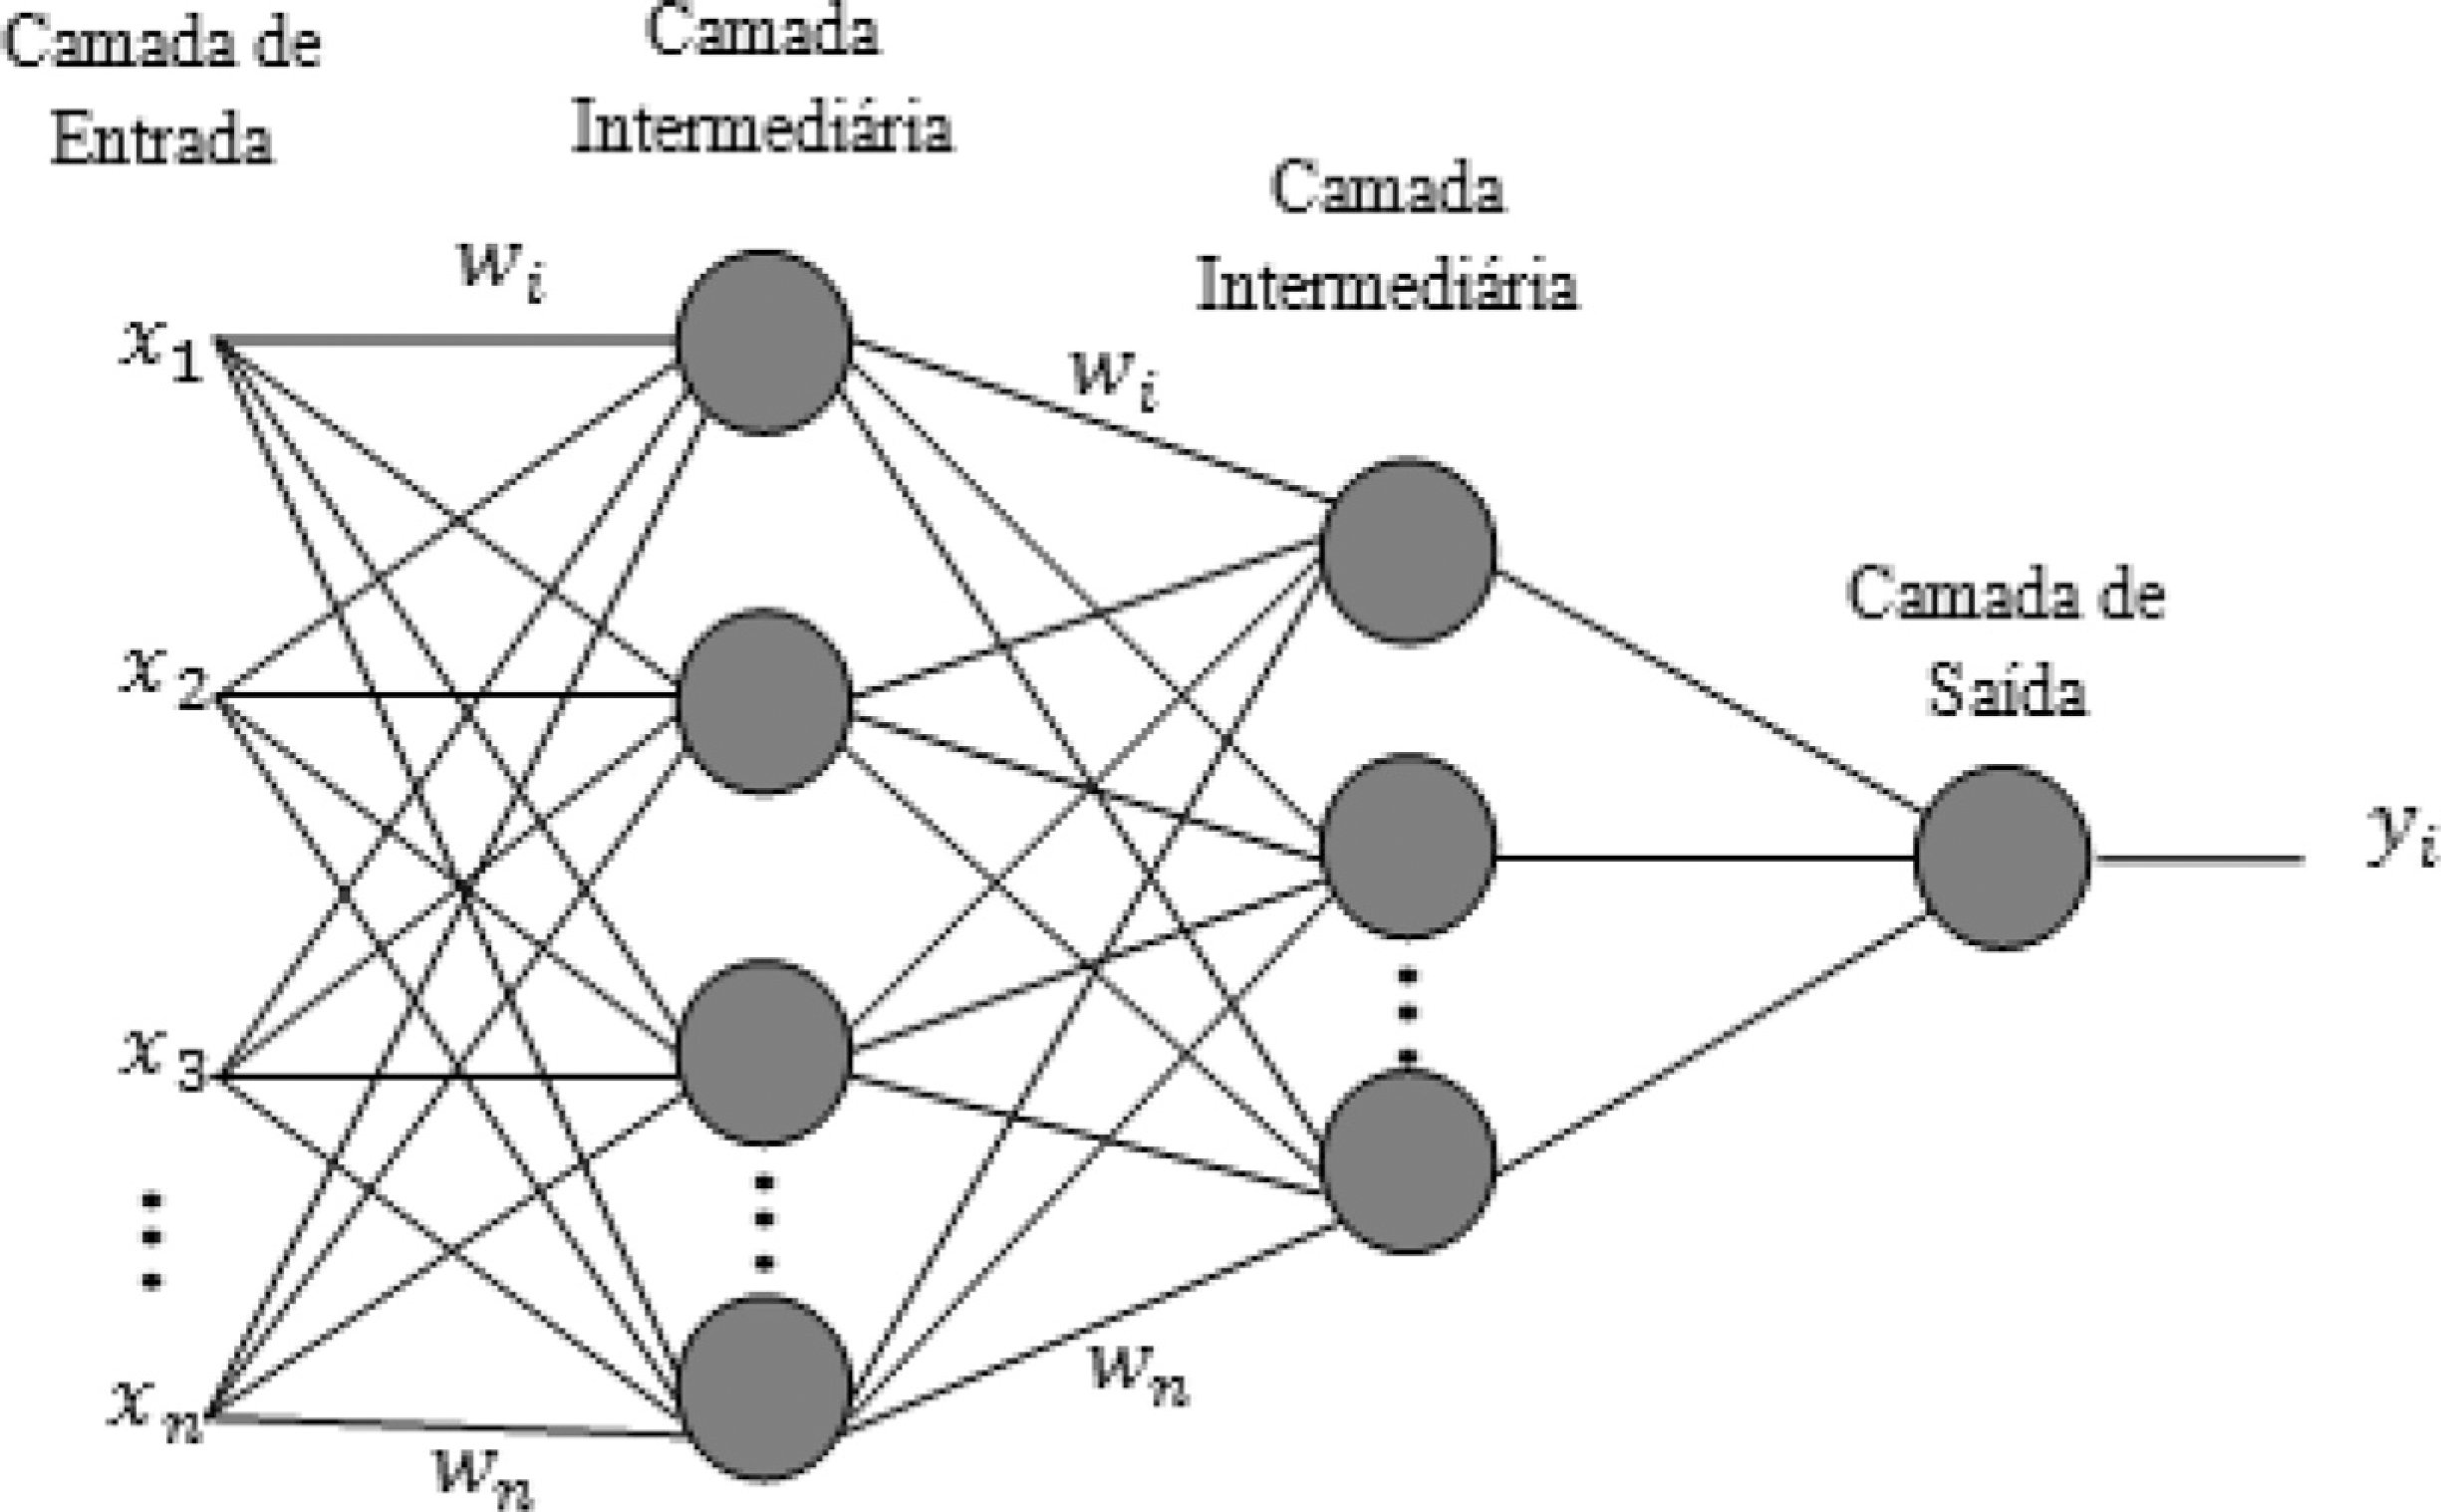
\includegraphics[width=0.7\textwidth]{img/mlprna.jpg}
	\caption{Rede Neural Multicamadas}
	\label{fig:mlp}
\end{figure}

Várias funções de ativação são utilizadas para determinar as saídas dos neurônios das camadas escondidas e de saída. As funções de ativação mais comuns são a linear ou identidade, \emph{ReLU} -- unidade exponencial linear retificada e suas variações, softmax, tangente hiperbólica e sigmoide.
%!TEX root = ../sbc-template.tex

\begin{table}[ht]
	\scalefont{0.8}
	\centering
	\caption{Funçoes de ativação mais populares. ---melhorar legenda}
	\label{tab:ativacoes}
	\begin{tabular}{l l p{6.5cm} l}
		\toprule
		Nome 			 		& Gráfico & Equação & Intervalo\\
		\midrule
		Identidade ou Linear		&
		 	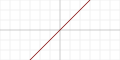
\includegraphics[width=0.1\textwidth]{img/identidade.png}
			&
			$
				\begin{aligned}
					g(z) = z
				\end{aligned}
			$
			& $(-\infty, + \infty) $\\
		\hline
		Tangente Hiperbólica		&
			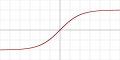
\includegraphics[width=0.1\textwidth]{img/tanh.png}
			&
			$
				\begin{aligned}
					g(z) = tanh(z) =\frac{(e^z - e^{-z})}{(e^z + e^{-z})}
				\end{aligned}
			$
			 & $(-1,1)$\\
		\hline
		Sigmoide ou Logística		&
			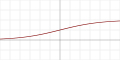
\includegraphics[width=0.1\textwidth]{img/sigmoid.png}
			&
			$
				\begin{aligned}
					g(z) = \sigma(z) = \frac{1}{1+e^{-x}}
				\end{aligned}
			$
			& $ (0,1) $\\
		\hline
		Unidade Linear Retificada	&
			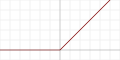
\includegraphics[width=0.1\textwidth]{img/relu.png}
			&
			$
				\begin{aligned}
					g(z) = max(0,z)
				\end{aligned}
			$
			& $ [0, \infty) $\\
		\hline
		Softmax					&
			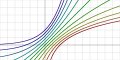
\includegraphics[width=0.1\textwidth]{img/softmax.png}
			&
			$
				\begin{aligned}
					g(\alpha, z) =
						\begin{cases}
							-\frac{ln(1-\alpha(z+\alpha))}{\alpha}, & \text{se } \alpha < 0\\
							z, & \text{se } \alpha = 0 \\
							\frac{e^{\alpha z} -1}{\alpha} + \alpha, & \text{se } \alpha > 0
						\end{cases}
				\end{aligned}
			$
			& $(-\infty, \infty)$\\
		\bottomrule
	\end{tabular}
\end{table}
. Todas estas alterações feitas ao modelo Perceptron inicial acabou por aumentar o escopo dos problema que podem ser resolvidos com RNAs.

\todo[inline]{aplicações}

As RNAs \emph{feedforward} formam a base para muitas aplicações, o que faz com que este modelo seja de extrema importância para profissionais da área de ML. Para exemplificar, as RNA convolucionais utilizadas para reconhecimento de objetos a partir de imagens são um tipo de RNAs \emph{feedforward}. Estas redes também são um pilar para as redes recorrentes, que alimentam muitas aplicações de linguagens naturais \cite{goodfellow2016deep}. Estes modelos filhos das RNAs \emph{feedforward} são parte da sub-área \emph{Deep Learning}, que será tratada na Seção \ref{sec:dl}.
